\subsection{Rematch using Quad Scan results}

During the machine setup the Twiss parameters were measured with the help of OTR screens~\ref{01_MTV}
using the quadrupole-scan technique, see Section~\ref{03_2_QuadScans}. 
The screens were installed at ten different positions along the machine. 
The measured parameters were used in the machine model to plot the optical functions
downstream and upstream of the measurement point. 
If the measured values were unsatisfactory a set of upstream quadrupoles was rematched to correct the error.
Usually two or three iterations were needed to approach the requested 
\textalpha~ and \textbeta~ values within 20\% precision.



\subsubsection{Middle of the Linac \tb{(girder 10)}}

Additionally to optics corrections this screen was used to optimise the injector emittance. 
It was done through adjusting the RF phases of the injector and the strength of the solenoids. 
The optics in the linac was corrected through back propagating the parameters to girder 6 and 
than model rematch from this location. Attempts to re-match from girder 4 were less effective. 
We believe that modelling of the edge focusing in the travelling wave cavities at low energy
(below 30~MeV) was not precise enough.
Another complication was a precise determination of the beam energy profile along the linac. 
Spectrometers in the injector and in the middle of the linac allowed to measure it precisely.  
For each of the accelerating cavities the energy gain was calculated from 
the measured RF-power that was not very accurate. 
Using these the energy profile was calculated with accuracy of a few~MeV. 

\subsubsection{CT Line (girder 15)}

The measured Twiss parameters were back propagated to the beginning of the CT line
and the quadrupole triplet in front of the Stretching Chicane was rematched.
If error was big quadrupoles at the end of the linac as well as the ones
at the start of the Stretching Chicane were employed.

It was observed that the measurements at this location sometimes 
varied for different quad ranges what was never explained.
Additionally, the results were in discrepancy with the measurements of 
the following screen in CTS, which was relatively close and separated
by only four quadrupoles. That is why its measurement were considered 
as not reliable and in practice it was rarely used.

\todo[inline]{find a two different emittances but different range}


%%%%%%%%%%%%%%%%%%%%%%%%%%%%%%%%%%%%%%%%%%%%%%%%%%%%%%%%%%%%%%%%%
\subsubsection{CTS Line}
\tb{Davide Thesis}

The measurements in CTS Line were crucial to
ensure the transverse optics matching of the recombined beams in the Delay Loop.
Figure~\ref{fig:trasverseDLmatchingAttempt} shows the quadrupole scan  data obtained before and after
an attempt to match the horizontal transverse optics of the delayed and bypassing beams.
The beam used was a nominal 1.5~GHz beam magnetically injected, or not, into the DL. 
%
\begin{figure}[htbp]
\centering
\subfloat[Before rematching.]{
\includegraphics[width=0.45\textwidth]{DLopticsClosurebeforeRematching15ghzH.eps}
\label{fig:trasverseDLmatchingAttemptBefore}
}
\qquad
\subfloat[After rematching.]{
\includegraphics[width=0.45\textwidth]{DLopticsClosureafterRematching15ghzH.eps}
\label{fig:trasverseDLmatchingAttemptAfter}
}
\caption{Horizontal beam variance measured at the screen CT.MTV0550 in the CTS dump line as a function
         of the quadrupole current used to perform quadrupole scan measurements before
         \protect\subref{fig:trasverseDLmatchingAttemptBefore} and after
         \protect\subref{fig:trasverseDLmatchingAttemptAfter} a first optics rematching at the end of
         the CTF3 linac.
         The error bars are computed from the Gaussian fits to the profiles measured at the screen.
         The dashed lines are the fits to the data corresponding to the Twiss parameters that are
         reported in Table~\ref{tab:quadMatchingDLfirst}.
         In blue are the measurements performed on a beam being delayed in the DL, while red
         represents the beam bypassing the DL.
}
\label{fig:trasverseDLmatchingAttempt}
\end{figure}
%
The rematching procedure used was to adjust the quadrupoles before the DL such that the beam would
arrive at the DL injection with the expected closed solution of the ring.
%The hope was that no major errors in the DL optics would change the theoretical closed solution of the ring.
%In fact the nominal optics of the DL could be adjusted easily by acting on the quadrupoles located in the dispersion-free quadrupoles.
%The new DL optics, which was in use during the measurements, does not allow one to easy correction because all the quadrupoles  
% more difficult tohas more constraints due to   one to correct only the delayed beam.
The Twiss parameters obtained for the two beams before and after the rematching are shown in
Table~\ref{tab:quadMatchingDLfirst}.
%
\begin{table}[htbp]
\centering
\begin{tabular}{l c c c | c c c}
\hline
               & \multicolumn{3}{c|}{Before correction}              & \multicolumn{3}{c}{After correction} \\
\hline
                & $\beta_x$  [m]  &  $\alpha_x$     &  $\epsilon_{Nx}$   [$\mu$m]   & $\beta_x$  [m]  &  $\alpha_x$     &  $\epsilon_{Nx}$   [$\mu$m] \\
\hline
Nominal values  & $8.4$           & $-0.8$          & --             & $8.4$       & $-0.8$       & --    \\
Bypass beam     & $13.2 \pm 0.6$  & $-0.9 \pm 0.1$  & $117 \pm 3$    & $5.9 \pm 0.3$   & $-0.6 \pm 0.1$   & $84 \pm 2$ \\
Delayed beam    & $10.5 \pm 0.4$  & $-1.3 \pm 0.1$  & $138 \pm 3$    & $6.8 \pm 0.5$   & $-0.5 \pm 0.1$   & $120 \pm 4$ \\
\hline 
\end{tabular}
\caption{Summary of the horizontal Twiss parameters measured in the CTS dump line for a beam bypassing
         the DL and one delayed in it.
         The first macro column contains the values before any optics correction, while the second
         macro column contains the values after a transverse optics matching between delayed and
         bypassing beams.}
\label{tab:quadMatchingDLfirst}
\end{table}
%
Note that in Figure~\ref{fig:trasverseDLmatchingAttempt}\subref{fig:trasverseDLmatchingAttemptBefore}
the minimum beam size is obtained for different values of the quadrupole used for the scan, while in
Figure~\ref{fig:trasverseDLmatchingAttempt}\subref{fig:trasverseDLmatchingAttemptAfter} both parabolas
are centred around the same minimum.
This is reflected in a better matching of the \textbeta~ and \textalpha~ parameters reported in
Table~\ref{tab:quadMatchingDLfirst}.
The measured emittance reduction was unexpected, especially for the bypassing beam.
From Figure~\ref{fig:trasverseDLmatchingAttempt} the emittance reduction is naively caused by the
overall smaller beam variance measured during the scan.

The parameters measured and reported in Table~\ref{tab:quadMatchingDLfirst} were not compatible a
priori with the desired nominal values.
A second iteration of re-matching was attempted. This time also the vertical plane was considered.
Figure~\ref{fig:trasverseDLmatchingFinal} shows similar quadrupole scan measurement obtained after the
last correction iteration.
%
\begin{figure}[hbp]
\centering
\subfloat[Horizontal]{
\includegraphics[width=0.45\textwidth]{DLopticsClosurefinalBeam15ghzH.eps}
\label{fig:trasverseDLmatchingFinalH}
}
\qquad
\subfloat[Vertical]{
\includegraphics[width=0.45\textwidth]{DLopticsClosurefinalBeam15ghzV.eps}
\label{fig:trasverseDLmatchingFinalV}
}
\caption{Beam variance measured at the screen CT.MTV0550 in the CTS dump line as a function of the
         quadrupole current used to perform quadrupole scan measurements 
         in the horizontal \protect\subref{fig:trasverseDLmatchingFinalH} and vertical
         \protect\subref{fig:trasverseDLmatchingFinalV} plane after optics rematching between bypass
         (red) and delayed (blue) beams.
         The error bars are computed from the Gaussian fits to the profiles measured at the screen.
         The dashed lines are the fits to the data corresponding to the Twiss parameters that are
         reported in Table~\ref{tab:quadMatchingDL}.
}
\label{fig:trasverseDLmatchingFinal}
\end{figure}
%
The final Twiss parameters for the different beams and planes are summarised in Table~\ref{tab:quadMatchingDL}.
%
\begin{table}[htbp]
\centering
\begin{tabular}{l c c c c c c}
\hline
              & $\beta_x$  [m]  &  $\alpha_x$     &  $\epsilon_{Nx}$   [$\mu$m]   & $\beta_y$  [m]  &  $\alpha_y$     &  $\epsilon_{Ny}$   [$\mu$m]    \\
\hline
Nominal values         & $8.4$       & $-0.8$       & --             & $13.5$       & $-0.4$       & -- \\
Bypass beam           & $7.6 \pm 1.0$   & $-0.8 \pm 0.1$   & $102 \pm 6$         & $4.6 \pm 0.3$  & $0.0 \pm 0.1$  &  $65 \pm 2$ \\
Delayed beam          & $8.9 \pm 1.1$   & $-0.6 \pm 0.1$   & $111 \pm 7$         & $2.7 \pm 0.3$  & $0.1 \pm 0.1$  &  $61 \pm 5$ \\
\hline 
\end{tabular}
\caption{Summary of the transverse Twiss parameters of the bypassing and delayed beams fitted from 
         the quadrupole scan measurements presented in Figure~\ref{fig:trasverseDLmatchingFinal}.}
\label{tab:quadMatchingDL}
\end{table}
%
One can see that in the horizontal plane the two beams seem to be reasonably matched with respect to
each other and close to the nominal values.
However in the vertical plane the results differ from the matching goal.

In order to better investigate what was happening it is useful to use the tomography technique
presented in Section~\ref{QuadScanTomo}.
The same profiles acquired to perform the quadrupole scan measurements shown in
Figure~\ref{fig:trasverseDLmatchingFinal} are used to produce 
the phase-space beam distribution reconstruction presented in Figure~\ref{fig:trasverseDLtomography}.
%
\begin{figure}[htbp]
\centering
\subfloat[Horizontal quadscan]{
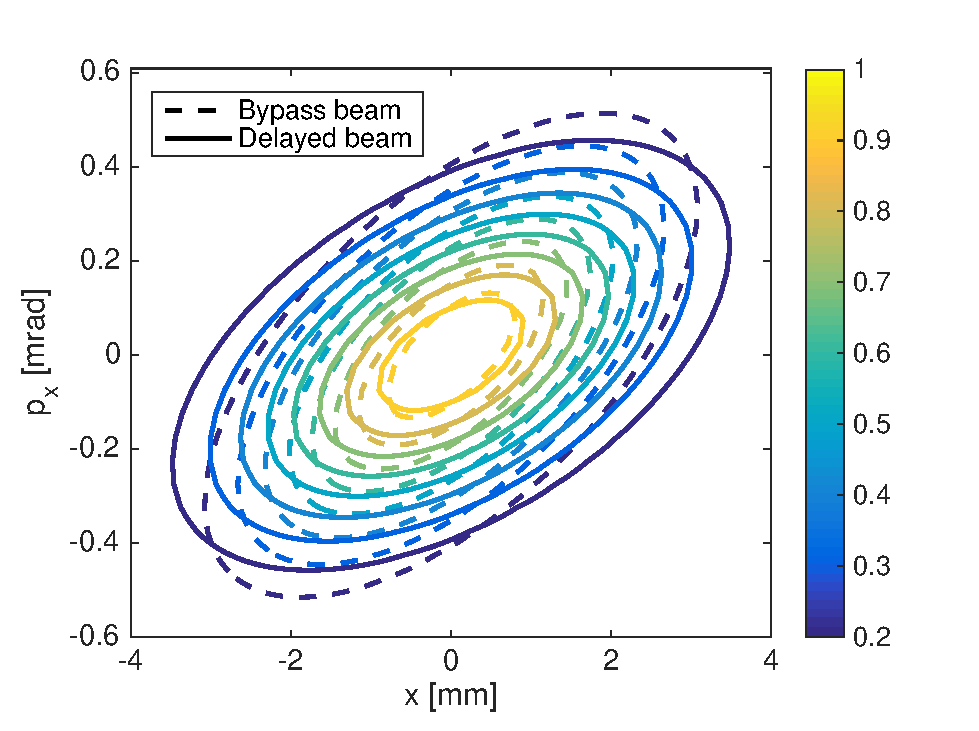
\includegraphics[width=0.45\textwidth]{DLopticsClosurefinalBeam15ghzH_quadscanTomoCentred.eps}
\label{fig:trasverseDLtomographyHQ}
}
\qquad
\subfloat[Horizontal tomography]{
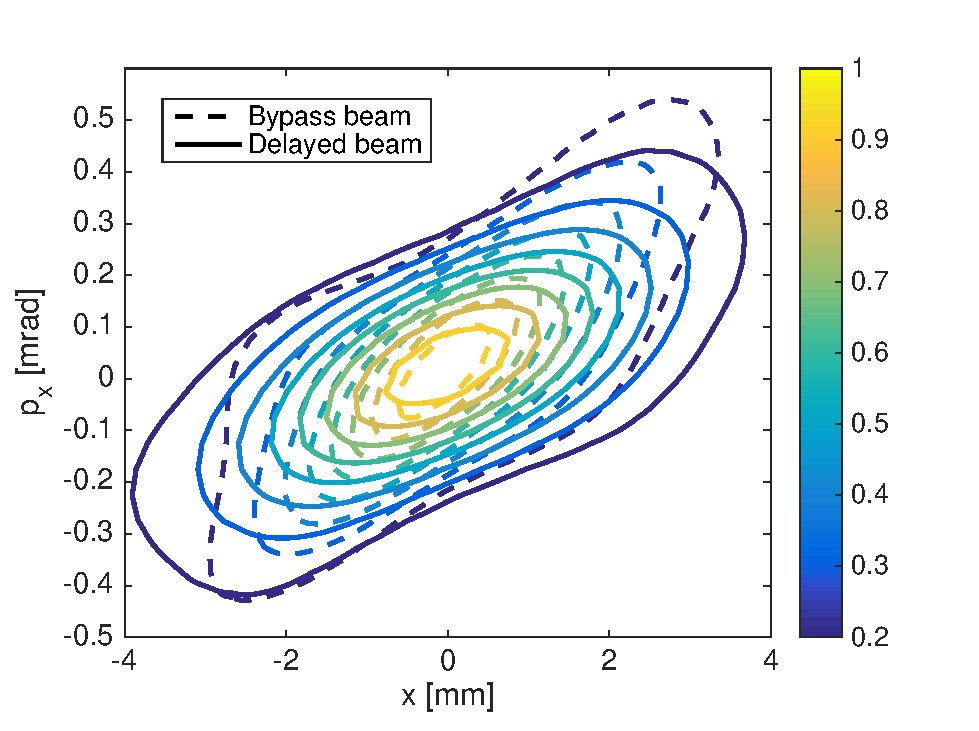
\includegraphics[width=0.45\textwidth]{DLopticsClosurefinalBeam15ghzH_tomo_biGaussianFit.eps}
\label{fig:trasverseDLtomographyHT}
}
\\
\subfloat[Vertical quadscan]{
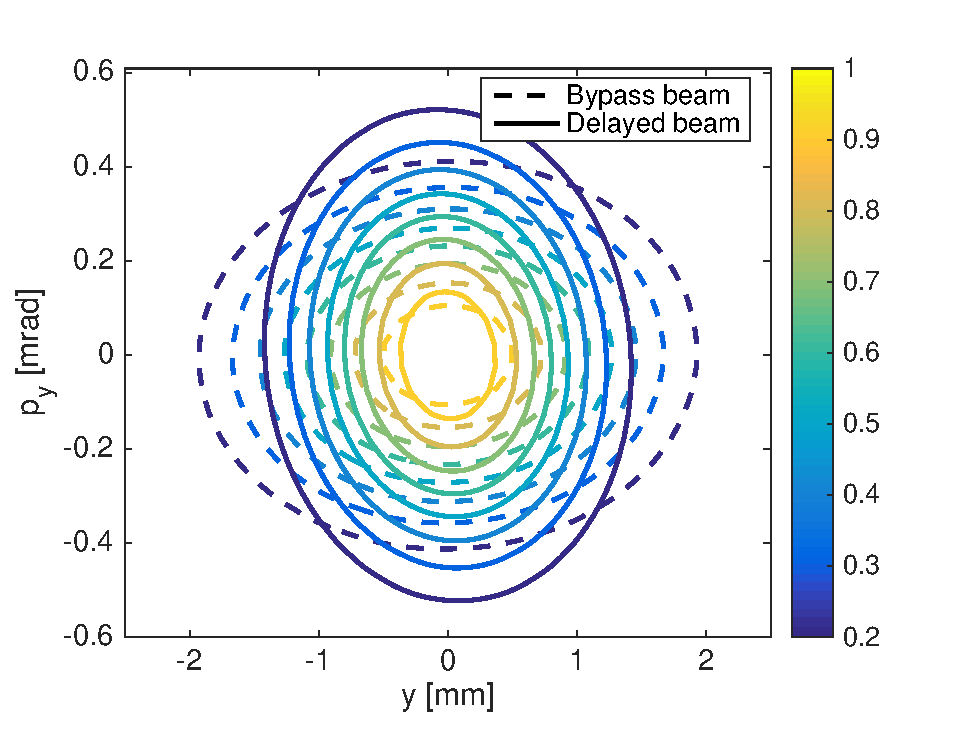
\includegraphics[width=0.45\textwidth]{DLopticsClosurefinalBeam15ghzV_quadscanTomoCentred.eps}
\label{fig:trasverseDLtomographyVQ}
}
\qquad
\subfloat[Vertical tomography]{
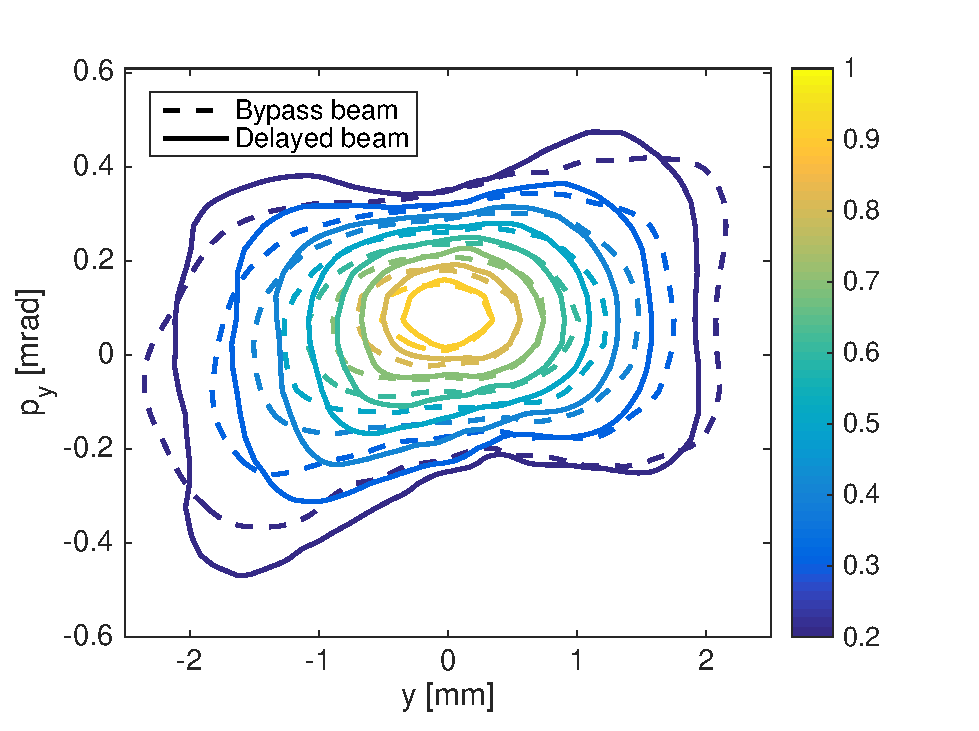
\includegraphics[width=0.45\textwidth]{DLopticsClosurefinalBeam15ghzV_tomo.eps}
\label{fig:trasverseDLtomographyVT}
}
\caption{Horizontal (\protect\subref{fig:trasverseDLtomographyHQ} and
         \protect\subref{fig:trasverseDLtomographyHT}) and vertical
         (\protect\subref{fig:trasverseDLtomographyVQ} and
         \protect\subref{fig:trasverseDLtomographyVT}) 
         phase-space distributions of the delayed and bypassing beams as measured by simple quadrupole
         scan (\protect\subref{fig:trasverseDLtomographyHQ} and
         \protect\subref{fig:trasverseDLtomographyVQ}) and tomographic
         (\protect\subref{fig:trasverseDLtomographyHT} and
         \protect\subref{fig:trasverseDLtomographyVT}) techniques.
         For both kinds of representation the same measured profile are used.
         The dashed contours represent the beam bypassing the DL, while the continuous ones are the
         distributions of the delayed beam.
         The colour code is the density distribution, which has been normalised to have a peak value
         equal to 1.
}
\label{fig:trasverseDLtomography}
\end{figure}
%
Indeed from the tomography view, especially in the vertical plane, it seems that the beam was far from
being Gaussian.
This leads to a difficult interpretation of the $\beta$ and $\alpha$ parameters measured with a
conventional quadrupole scan.
However the tomography reconstruction of the phase space suggests that the two beams are pretty well
matched with respect to each other, and the vertical $\beta$ parameter difference noted in
Table~\ref{tab:quadMatchingDL} might actually be harmless.
Still the non-Gaussian shape of the phase space might be a limiting factor for the overall performance
of the DBRC. 
A dedicated study would be needed to verify the accuracy and precision of the tomographic
measurements, which has not been performed yet.


